\documentclass[border=10pt]{standalone}

\usepackage[utf8]{inputenc}                                 % Codificação do documento
\usepackage[T1]{fontenc}                                    % Seleção de código de fonte
\usepackage{microtype}                                      % Melhora a justificação do documento
\usepackage{lmodern}                                        % Usa a fonte Latin Modern
\usepackage{ae, aecompl}                                    % Fontes de alta qualidade

\usepackage{amsmath}
\usepackage{verbatim}
\usepackage{tikz}
\usetikzlibrary{arrows,calc,positioning,shadows.blur,decorations.pathreplacing}
\usepackage{etoolbox}

\begin{document}
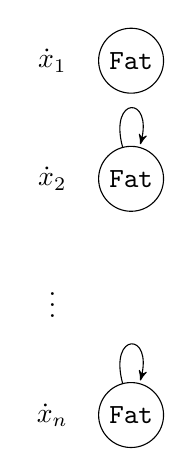
\begin{tikzpicture}
[
	              y = -1cm,
	           ->, >= stealth',
	  node distance = 2cm,
	  vertex/.style = { draw=black, circle, inner sep=2.5pt },
	   label/.style = { draw=none, fill=none },
	toplabel/.style = { label, anchor=south }
]
	\node (50) at  (8,0)    [label]    {$\dot{x}_1$};
	\node (51) at  (9,0)    [vertex]   {\texttt{Fat}};

	\node (60) at  (8,1.5)  [label]    {$\dot{x}_2$};
	\node (61) at  (9,1.5)  [vertex]   {\texttt{Fat}};
	\draw [->] (61) edge [loop above] (61);

	\node (70) at  (8,3)    [label]    {$\vdots$};

	\node (80) at  (8,4.5)  [label]    {$\dot{x}_n$};
	\node (81) at  (9,4.5)  [vertex]   {\texttt{Fat}};
	\draw [->] (81) edge [loop above] (81);

\end{tikzpicture}
\end{document}